\documentclass[a4paper,11pt]{article}
\newcommand\tab[1][0.6cm]{\hspace*{#1}}
\usepackage{mlsubmit}
\usepackage{amsmath}
\newenvironment{absolutelynopagebreak}
  {\par\nobreak\vfil\penalty0\vfilneg
   \vtop\bgroup}
  {\par\xdef\tpd{\the\prevdepth}\egroup
   \prevdepth=\tpd}
\raggedbottom

\begin{document}

\title{MATH578A Assignment 1 }
\author{Raktim Mitra \\ \small{USC ID: 1487079265\hspace{10pt} email: raktimmi@usc.edu}}
\maketitle
\initmlsubmision{1}                              					% assignment number
								{Raktim Mitra}      						           		% your name
								{150562}																		% your roll number
								
\section*{Q1. }
I chose Rabbit (Oryctolagus cuniculus) genome downloaded from NCBI genome page for rabbit. (\url{https://www.ncbi.nlm.nih.gov/genome/?term=Oryctolagus+cuniculus}).

Total number of sequences in fasta file : 3241

Number of base pairs: 2771682684

Results on the test pattern searches on rabbit genome are as follows:
\begin{center}
\begin{tabular}{ | c | c | c | c |}
\hline
Pattern & Occurence & comparisons & runtime(seconds) \\ 
\hline
\hline
 \scriptsize{{ACACACACACACACACACACACACACACACACACACACAC}} & 614 & 539841559 & 12.111216\\
 \hline
 \scriptsize{GAGAGAGAGAGAGAGAGAGAGAGAGAGAGAGAGAGAGAGA} & 15195 & 473455211 & 9.997119\\  
 \hline
 \scriptsize{CAGCAGCAGCAGCAGCAGCAGCAGCAGCAGCAGCAGCAGC} & 10 & 524563641 & 12.610945\\   
\hline
 \scriptsize{GACGACGACGACGACGACGACGACGACGACGACGACGACG} & 0 & 523252832 & 13.063918\\  
 \hline
 \scriptsize{ACAGACAGACAGACAGACAGACAGACAGACAGACAGACAG} & 1 & 507595359 & 11.662198\\   
\hline
\scriptsize{AACGAACGAACGAACGAACGAACGAACGAACGAACGAACG} & 0 & 523598924 & 12.964050\\
 \hline
 \scriptsize{AAGCAAGCAAGCAAGCAAGCAAGCAAGCAAGCAAGCAAGC} & 1 & 525172676 & 12.699295\\  
 \hline
 \scriptsize{CCACCAGGGG} & 4037 & 1206400435 & 31.577522\\   
\hline
\scriptsize{GGAGGACCCC} & 2648 & 1188278808 & 30.708362\\   
\hline
 \end{tabular}
\end{center}

Results on the test sequences on HG38 (human genome) taken from (\url{https://www.ncbi.nlm.nih.gov/genome/?term=Homo+sapiens}):
\begin{center}
\begin{tabular}{ | c | c | c | c |}
\hline
Pattern & Occurence & comparisons & runtime(seconds) \\ 
\hline
\hline
 \scriptsize{{ACACACACACACACACACACACACACACACACACACACAC}} & 27877 & 667532560 & 15.362110\\
 \hline
 \scriptsize{GAGAGAGAGAGAGAGAGAGAGAGAGAGAGAGAGAGAGAGA} & 4365 & 544768912 & 11.428859\\  
 \hline
 \scriptsize{CAGCAGCAGCAGCAGCAGCAGCAGCAGCAGCAGCAGCAGC} & 103 & 643608461 & 15.230797\\   
\hline
 \scriptsize{GACGACGACGACGACGACGACGACGACGACGACGACGACG} & 7 & 640093906 & 15.678619\\  
 \hline
 \scriptsize{ACAGACAGACAGACAGACAGACAGACAGACAGACAGACAG} & 31 & 628499838 & 14.257126\\   
\hline
\scriptsize{AACGAACGAACGAACGAACGAACGAACGAACGAACGAACG} & 0 & 640427323 & 15.587231\\
 \hline
 \scriptsize{AAGCAAGCAAGCAAGCAAGCAAGCAAGCAAGCAAGCAAGC} & 45 & 645121107 & 15.222942\\  
 \hline
 \scriptsize{CCACCAGGGG} & 3391 & 1449562317 & 36.682713\\   
\hline
\scriptsize{GGAGGACCCC} & 2437 & 1423537154 & 36.751045\\   
\hline
 \end{tabular}
\end{center}
Chosen ALU sequence: {\scriptsize{``GGCGGGCAGATCATGAGGTCAGGAGATCGAGACCATCCTGGCTAACACGG''}}.\\
In Hg38, Total Matches found:	117\\
Char comparisons:	1014339834\\
Time taken in seconds:	30.342192\\

\begin{center}
 -------------------
\end{center}

\section*{Q2. (Chapter 1, exercise 11)}
\textbf{Q}: Let T be a text string of length m and let S be a multiset of n characters. The problem is
to find all substrings in T of length n that are formed by the characters of S. For example,
let S = \{a, a, b, c\} and T = `abahgcabah'. Then `caba' is a substring of T formed from the
characters of 5.
Give a solution to this problem that runs in O(m) time. The method should also be able to
state, for each position i, the length of the longest substring in T starting at i that can be
formed from S.
\\
\\
\textbf{Ans}: Let, A[ ] contains unique elements of S. Count[ ] array contains number of occurences of each element of A in S.
\\

Now, we shall construct the array D[ ] where D[i] contains length of the longest substring of T that \underbar{ends} at position i which can be formed by elements from S.
\\
i ranges from 0 to m-1. 
\\
\\
We also need a RunningCount[ ] array similar to Count[ ], which will use to keep track of counts of elements of S faced for D[i].
A, Count, RunningCount all have the length count(unique(S)).
Note: A.index[c] gives position of char c in A, constant time since A is of constant length assuming alphabet size is constant. 
Therefore, we can write the following recurrence for D[i].
\[D[i] = \begin{cases}
          0 \text{ if T[i] is not in A (case 1)} \\
          \text{ if T[i] is in A }\begin{cases}
          D[i-1] + 1 &\text{ if RunningCount[A.index[T[i]]] $<$ Count[A.index[T[i]]]} \\&\text{($\uparrow$ case 2a)} \\
          i - j &\text{ if RunningCount[A.index[T[i]]] $==$ Count[A.index[T[i]]] }\\
          &\text{where j is the first occurence of T[i] after i - 1 - D[i-1] }\\&\text{($\uparrow$ case 2b)} \\
          \end{cases} \\ 
         \end{cases}
    \]

For the above recurrence to work properly , we need to update RunningCount in the following manner:
\[\begin{cases}
            \text{ (case 1) RunningCount[i] = 0 for all i  } \\
          \begin{cases}
           \text{ (case 2a) RunningCount[A.index[T[i]]] += 1} \\
          \text{ (case2b)  RunningCount[A.index[T[k]]] $-$= 1, for k in interval (i,j) }\\
          
          \end{cases} \\ 
         \end{cases}
         \] \\
         
After we fill up the array D we can report all starting occurence position as: \{i - size(S) for  i if D[i] == size(S)\}.
\begin{center}
 P.T.O.
\end{center}

\begin{absolutelynopagebreak}
{We can also construct length of longest substrings \underbar{starting} at i and formed by elements of S from D. Let, this array be B[ ]. Shown in full pseudocode below:}
\end{absolutelynopagebreak}
\begin{mlalgorithm}[0.9\textwidth]{H}{Multiset Matching }\vskip-2ex
	\label{algo:tk-means}
	\begin{algorithmic}[1]
		\REQUIRE Text T and Multiset S
		\STATE A $\leftarrow$ Unique(S)
		\STATE initialize Count[0...length(A)] to all 0
        \STATE initialize RunningCount[0...length(A)] to all 0
		\FOR{element e in S}
		\STATE  Count[A.index[e]]++
		\ENDFOR 
		\STATE intiailize D[0...m-1]
		\STATE D[-1] $\leftarrow$ 0 \COMMENT{For convenience, In actual implementation we would hardcode D[0] and start the following loop at 1.}
		\FOR{\{i=0; i $<$ m; i++\}}
            \IF [Case 1]{T[i] not in A } 
            \STATE D[i] $\leftarrow$ 0 
            \STATE \{RunningCount[j] $\leftarrow$ 0 for j in interval [0,length(a))\}
            \ELSIF{RunningCount[A.index[T[i]] $<$ Count[A.index[T[i]]]\COMMENT{Case 2a}} 
            \STATE D[i] $\leftarrow$ D[i-1] + 1 
            \STATE RunningCount[A.index[T[i]]++
            \ELSE [Case 2b]
            \STATE j $\leftarrow$ i - D[i-1] + 1 //Case 2b
            \WHILE{j$\leq$i and T[j] != T[i]}
            \STATE RunningCount[A.index[T[j]]]$--$
            \ENDWHILE
            \STATE D[i] $\leftarrow$ i $-$ j
            \ENDIF
		\ENDFOR
		\STATE Initialize B[0..m-1] \COMMENT{length of substrings longest substrings formed by elements of S from starting positions.}
		\STATE  i $\leftarrow$ 0
		\STATE  Initialize R \COMMENT{List of starting positions of occurences}
		\WHILE[O(m), only correct when i goes from 0 to m-1, the descending order of traversal won't work.]{\{i $<$ m\}} 
            \STATE B[i - D[i]] $\leftarrow$ D[i]
            \IF{D[i] == size(S)}
            \STATE R.add(i - D[i])
            \STATE i++
            \ENDIF
        \ENDWHILE
		\RETURN R, B
	\end{algorithmic}
\end{mlalgorithm}

\textbf{Time Complexity:} Clearly all the preprocessing can be done in O(m) time and so is generating R and B from D.

That leaves constructing D. The for loop (line 9-23) runs m times. Case 1 and Case 2a are clearly O(1) [Assuming alphabet size is O(1)]. However, the while loop (Case 2b, line 18-20) can be O(size(S)) in worst case. 
But, we can use amortized analysis to show that amortized cost of each iteration of the for loop is O(1). The reason is, case2b can decrement RunningCount (line 19) size(S) times only when Case(2a) has been executed size(S) times. (Because only Case 2a increments RunningCount (line 15).)

Therefore, Case 2b can be O(size(S)) only after O(size(s)) iterations of case 2b which are all O(1) iterations. Therefore, on average each iteration takes O(1), making the whole for loop O(m).

Hence, time complexity of Multiset Matching is O(m).
\begin{center}
 -------------------
\end{center}
\section*{Q3. (Chapter 6, exercise 1.)}
\textbf{Q}: Construct an infinite family of strings over a fixed alphabet, where the total length of the
edge-labels on their suffix trees grows faster than O(m) (m is the length of the string). That
is, show that linear-time suffix tree algorithms would be impossible if edge-labels were
written explicitly on the edges.
\\
\textbf{Ans}: Let, $B^k = BBB...B$ ($k$ times)
Then the following  family of strings over the alphabet $\Sigma = \{A,B\}$ is a required example. 
\begin{align*}
 S_n  &= AB^0AAB^1AAB^2A...AB^nA \\
 S_0 &= AA\\
 S_1 &= AAABA\\
 S_2 &= AAABAABBA\\
\end{align*}
Note: $S_n$ has length $(2 + 3 + 4 + ... + (n+2)) = \frac{(n+2)(n+3)}{2}-1 = O(n^2)$.\\Suffix trees for $S_0,S_1, S_2$:
\begin{figure}[H]

\centering
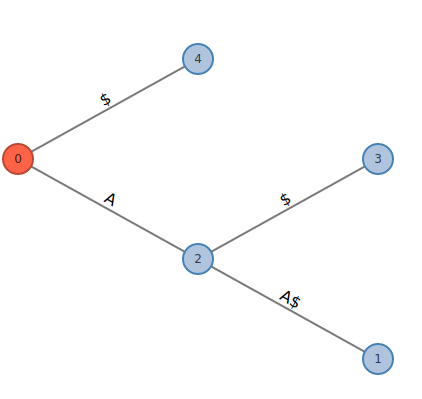
\includegraphics[width=.3\textwidth]{AA.png}\hfill
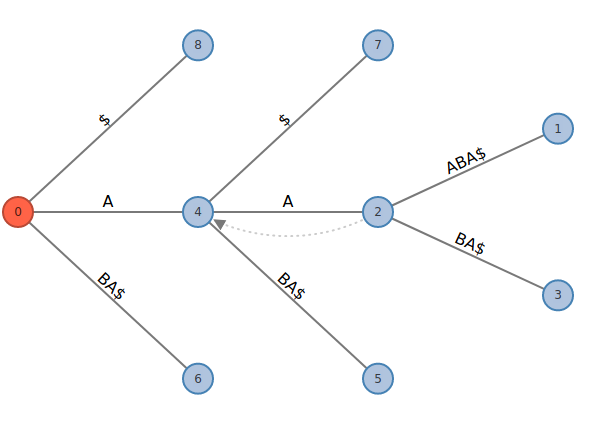
\includegraphics[width=.3\textwidth]{AAABA.png}\hfill
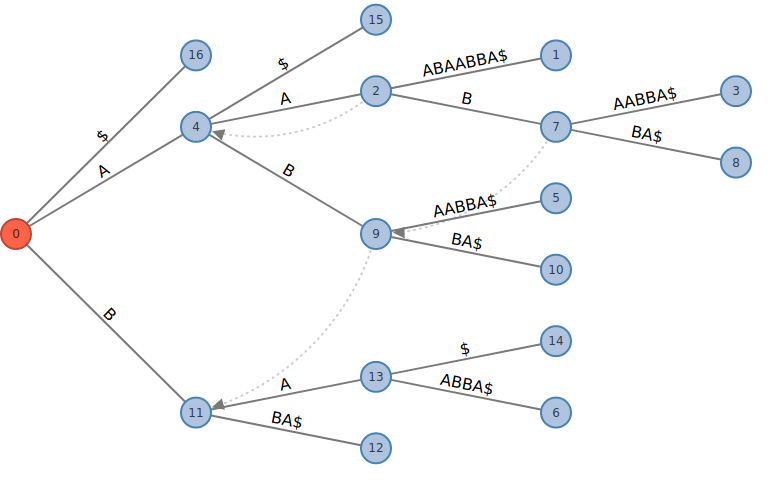
\includegraphics[width=.3\textwidth]{AAABAABBA.png}

\caption{suffix trees for AA, AAABA and AAABAABBA}

\label{fig:figure3}
\end{figure}
We can simply look at how total length of edge labels scales w.r.t lengths of $S_n$:
\begin{center}
\begin{tabular}{ | c | c | c | }
\hline
$n$ & length($S_n$) & total edge label length(excluding \$s) \\ 
\hline
\hline
 0 & 2 & 2\\
 \hline
 1 & 5 & 11 \\  
 \hline
 2 & 9 & 33 \\   
\hline
 \end{tabular}
\end{center}
Clearly total length of edge labels grows much faster than length of the strings.

It is impossible for an O(m) algorithm to write explicitely more than O(m) labels. So, it is not possible to have an O(m) algorithm if we are writing the edge labels explicitly. 
\begin{center}
 ------------------
\end{center}
\section*{Q4. (Chapter 7, exercise 1.)}
\textbf{Q}: Given a set S of k strings, we want to find every string in S that is a substring of some other string in S. Assuming that the total length of all the strings is n, give an O(n)-time algorithm to solve this problem. 
\\
\\
\textbf{Ans}: We can build a generalized suffix  tree $S_1\$_1S_2\$_2...S_k\$_k$ with k distinct terminal markers $\$_1,...,\$_k \notin \Sigma$ in linear time. We label leaves with (i,j) if they represent suffix $S_i[j..|S_i|]$. 

First we need to find all leaves labelled (i,0). Which takes one traversal i.e. linear time.

Now, for every leaf (i,0) go to it's parent reachable through an edge lablled $\$_i$. Find all leaves (j,0)  reachable from that node except (i,0). Return all such pairs (i,j) where $S_i$ appearing as a substring of $S_j$. This also takes linear time.



\begin{center}
-----------------\\
\end{center}

\section*{Q5. (Chapter 7, exercise 2.)}
\textbf{Q}: For a string S of length n, show how to compute the N(i), L(i), L'(i) and sp, values (discussed in Sections 2.2.4 and 2.3.2) in O(n) time directly from a suffix tree for S.
\\
\\
 \textbf{Ans}:  Using McCreight’s algorithm  we can build a suffix tree ST for (reverse of S) $S^r$ in linear time.
 
 \textbf{For N(i)}:
 N(i) values are Z-values of positions of $S^r$ in reverse order. i.e. $N_S$(i) = $Z_{S^r}$(n-i+1).
 We can compute $N_S$(i) using ST in the following manner:

 If we take the branch corresponding to the first character in $S^r$ and find all the leaves reachable through that branch, those are the positions (i.e. starting positions of the suffixes denoted by those leaves) in $S^r$ with non-zero $Z_{S^r}$ values. The value of  $Z_{S^r}(i)$ is the letter-depth of the node at which the path to leaf $i$ deviates from the path representing full string.
 
 Hence, we can initialize $Z_{S^r}(i) = 0$ for all $i$. Then we can update $Z_{S^r}(i)$ for all those leaves using one traversal through the branch corresponding to first letter in $S^r$ and update  those $Z_{S^r}(i)$ values. Then assign $N_S(n - i + 1) = Z_{S^r}(i)$ for all i. 
 
  \textbf{For L'(i)}:
 We can initialize $L'(i)_{S}(i) = 0$ for all $i$. Then we can follow the same procedure (using suffix tree for $S^r$ and traversing through the first letter branch of $S^r$.) as N(i) except the following change. Let, we reach leaf $i$ and path to leaf $i$ leaves the full reverse-string suffix path at a node with letter depth k. (note, this means, $N_S(n-i+1)=k$).  This means we can assign $L'(n-k+1) = n-j+1$  if $n-j+1$ is greater than older value. 
 
 [Note: Evident from this process, $L'_S(i)$ can be calculated from $N_S(i)$ in linear time too. Since, the maximisation is on index j of $S$ (n-j+1 on $S^r$) this can be done by going top down (from n to 0) through $N_S(i)$ and update L' accordingly.]
 
\textbf{For L(i)}:
After calculating L$'(i)$ from the suffix tree of $S^r$, L(i) values can be quickly calculated from the L$'(i)$ values. using the following recurrence:\\
L(2) = L$'(2)$ and    for (i=3 to n): L(i) = max(L(i-1),L$'(i)$) as described in Gusfield's book.

 \textbf{For SP(i)}:
 In this case we start from the suffix of tree of original string $S$. %This time leaves reachable through the branch toward $S[0]$ will have SP$'(i) \neq 0$ where SP' is as described in Gusfield section 2.3.1 .
 
 Let, path to leaf $i$ among leaves reachable through branch of $S[0]$ deviate from full string path at a node with letter depth $k$. Note, the common path bwteen path to leaf $i$ and full string path corresponds to a string of length ending at position $i = j + k - 1$ which is also a prefix of the full string (and the next characters are unequal since we encountered a branching.)
 Therefore,  we can assign SP$'(i) = k$ where SP$'(i)$ values are as described in Gusfield section 2.3.1 . 
 
 $SP'(i) = 0$ for all other leaves. Now, we can calculate SP values using the recurrence $SP(i) = max(SP(i+1)-1,SP'(i))$ .
 
% The structure of a suffix tree of S, implies ``The Z-score at position i of S is the depth of the parent of suffix i.''  

\begin{center}

 ------------------ -----------------
\end{center}

\end{document}
